% !TEX TS-program = pdflatex
% !TEX encoding = UTF-8 Unicode

\documentclass[1pt]{article} % use larger type; default would be 10pt

\usepackage[utf8]{inputenc} % set input encoding (not needed with XeLaTeX)


%%% PAGE DIMENSIONS
\usepackage{geometry} % to change the page dimensions
\geometry{a4paper} 
\geometry{margin=0.5in} 
% \geometry{landscape} 
%   read geometry.pdf for detailed page layout information


% \usepackage[parfill]{parskip} % Activate to begin paragraphs with an empty line rather than an indent

%%% PACKAGES
\usepackage{fancybox}
\usepackage{graphicx} 
\usepackage{booktabs} % for much better looking tables
\usepackage{array} % for better arrays (eg matrices) in maths
\usepackage{paralist} % very flexible & customisable lists (eg. enumerate/itemize, etc.)
\usepackage{verbatim} % adds environment for commenting out blocks of text & for better verbatim
\usepackage{subfig} % make it possible to include more than one captioned figure/table in a single float
% These packages are all incorporated in the memoir class to one degree or another...

%%% HEADERS & FOOTERS
\usepackage{fancyhdr} % This should be set AFTER setting up the page geometry
\pagestyle{fancy} % options: empty , plain , fancy
\renewcommand{\headrulewidth}{0pt} % customise the layout...
\lhead{}\chead{}\rhead{}
\lfoot{}\cfoot{\thepage}\rfoot{}

%%% SECTION TITLE APPEARANCE
\usepackage{sectsty}
\allsectionsfont{\sffamily\mdseries\upshape} % (See the fntguide.pdf for font help)
% (This matches ConTeXt defaults)

%%% ToC (table of contents) APPEARANCE
\usepackage[nottoc,notlof,notlot]{tocbibind} % Put the bibliography in the ToC
\usepackage[titles,subfigure]{tocloft} % Alter the style of the Table of Contents
\renewcommand{\cftsecfont}{\rmfamily\mdseries\upshape}
\renewcommand{\cftsecpagefont}{\rmfamily\mdseries\upshape} % No bold!

\title{Documentación LXC}
\author{García Silva Adán Alberto}
%\date{} % Activate to display a given date or no date (if empty),
         % otherwise the current date is printed 

\begin{document}
\maketitle

\section{Porqué LXC}

Hoy en día la tecnología de LinuX Containers (LXC) te permite crear contenedores que son servidores linux aislados, en tu máquina Linux real, estos contenedores comparten el kernel con la máquina principal. Es como una virtualización muy ligera, tan ligera que realmente no hay virtualización en absoluto por llamarlo así, y por lo tanto no tiene un impacto negativo en el rendimiento. En este artículo explicaré el funcionamiento de Linux Containers en base a experiencia documentada y crearé un contenedor observando el comportamiento del mismo en el entorno.
\\
\\
La tecnología LXC utiliza Linux kernel control groups (cgroups) y NameSpaces (espacios de nombres) para proporcionar este aislamiento. Cabe mencionar que 

\section{Instalación LXC}

Buscamos los paquetes disponibles para LXC mediante apt, obteniendo lo siguiente:
\begin{center}
	\shadowbox{ sudo apt-cache search lxc.}
\end{center}
\begin{figure}[!ht]
	\begin{center}
		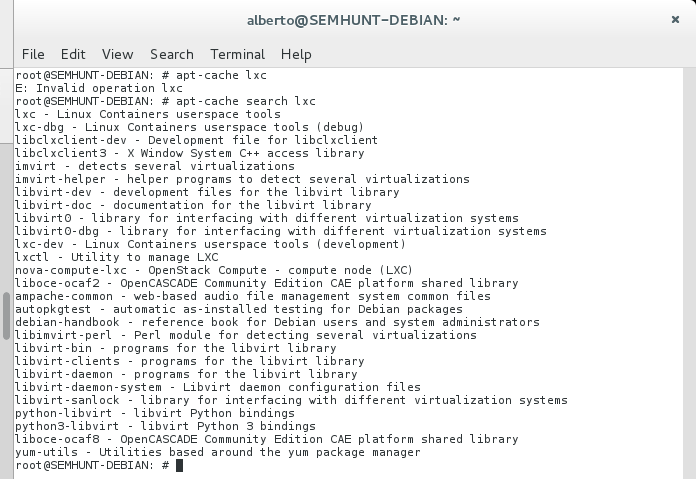
\includegraphics[width=0.9\textwidth]{1.png}
		\caption{Búsqueda de Paquetes LXC}
	\end{center}
\end{figure}

\newpage
\setlength{\parindent}{0em} 									%Quitamos la Identación
Posteriormente se procede a instalar lxc:

\begin{center}
	\shadowbox{ sudo apt-get install lxc bridge-utils libvirt-bin debootstrap.}
\end{center}
\begin{figure}[!ht]
	\begin{center}
		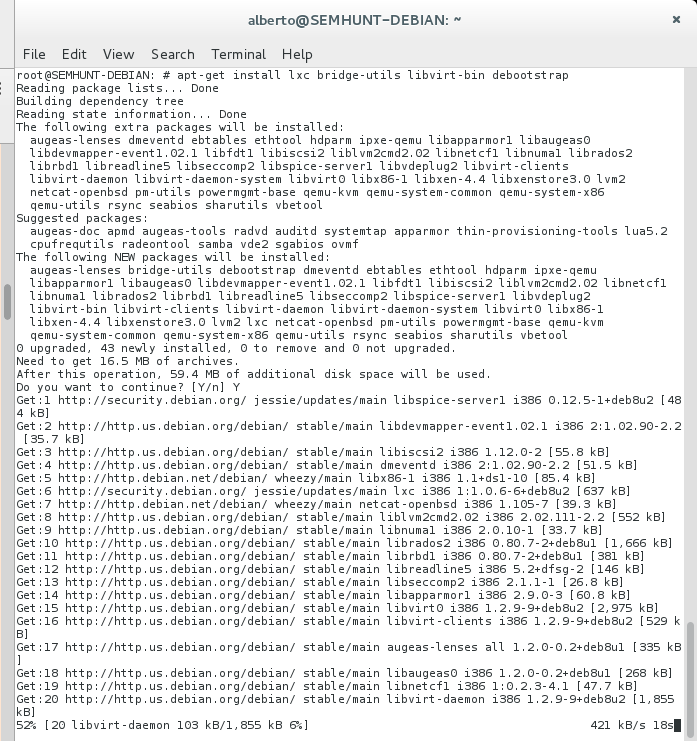
\includegraphics[width=0.9\textwidth]{3.png}
		\caption{Instalación LXC}
	\end{center}
\end{figure}
CGROUPS es una característica del kernel necesaria para que LXC corra apropiadamente. Comenzaremos agregandolos siguiente al archivo /etc/fstab y montarlos:

\begin{center}
	\shadowbox{ cgroup  /sys/fs/cgroup  cgroup  defaults  0   0.}
	\\
	\shadowbox{ sudo mount /sys/fs/cgroup.}
\end{center}

\newpage
\section{Creación de un Contenedor}

Podemos revisar que templates se encuentran disponibles en la version LXC instalada.

\begin{center}
	\shadowbox{ ls /usr/share/lxc/templates.}
\end{center}
\begin{figure}[!ht]
	\begin{center}
		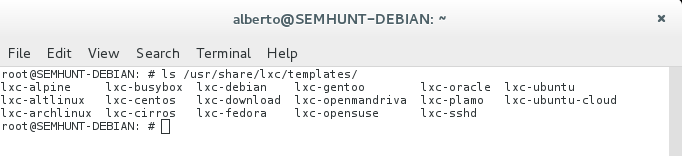
\includegraphics[width=0.9\textwidth]{7.png}
		\caption{Templates LXC}
	\end{center}
\end{figure}
Ahora se deberá ejecutar la siguiente sentencia para cada contenedor que se desee crear. Hagámos nuestro primer contenedor:

\begin{center}
	\shadowbox{ sudo lxc-create -n myfirstcontainer -t debian.}
\end{center}
\begin{figure}[!ht]
	\begin{center}
		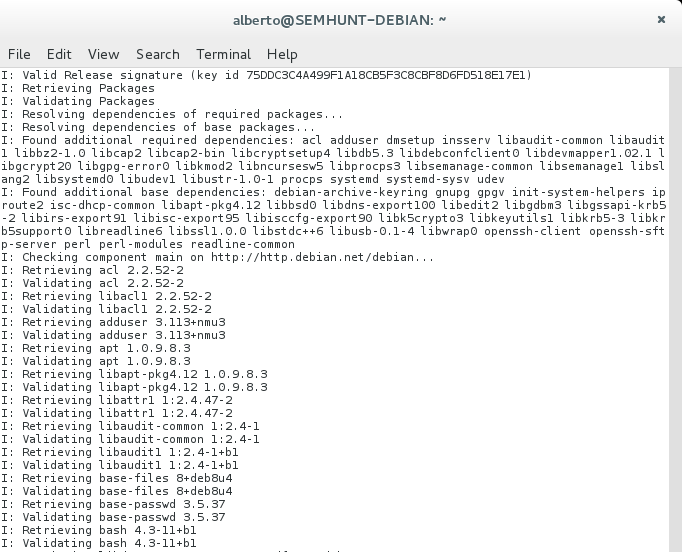
\includegraphics[width=0.9\textwidth]{8.png}
		\caption{Creación de Contenedor LXC}
	\end{center}
\end{figure}
\newpage
\begin{figure}[!ht]
	\begin{center}
		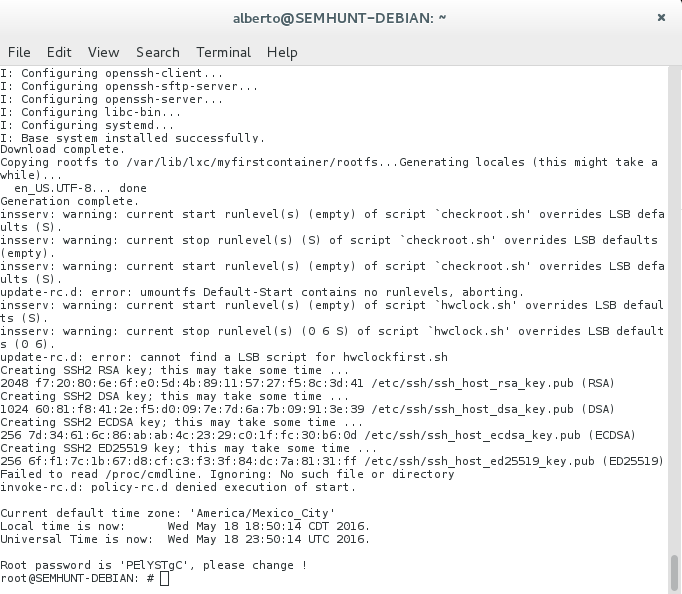
\includegraphics[width=0.9\textwidth]{11.png}
		\caption{Creación de Contenedor LXC}
	\end{center}
\end{figure}
Una vez que se crea el contenedor ( esto toma algún tiempo porque tiene que descargar todos los paquetes base e instalar un sistema base), chroot en ella y crear algunos dispositivos TTY . He descubierto que el comando lxc-console no funcionaba si yo no he creado estos dispositivos en primer lugar:

\begin{center}\shadowbox{ sudo chroot /var/lib/lxc/myfirstcontainer/rootfs.}\end{center}
\begin{center}\shadowbox{ mknod -m 666 /dev/tty1 c 4 1.}\end{center}
\begin{center}\shadowbox{ mknod -m 666 /dev/tty2 c 4 2.}\end{center}
\begin{center}\shadowbox{ mknod -m 666 /dev/tty3 c 4 3.}\end{center}
\begin{center}\shadowbox{ mknod -m 666 /dev/tty4 c 4 4.}\end{center}
\begin{center}\shadowbox{ mknod -m 666 /dev/tty5 c 4 5.}\end{center}
\begin{center}\shadowbox{ mknod -m 666 /dev/tty6 c 4 6.}\end{center}

\newpage

Ahora iniciamos el contenedor:

\begin{center}\shadowbox{ sudo lxc-start -n myfirstcontainer.}\end{center}
\begin{figure}[!ht]
	\begin{center}
		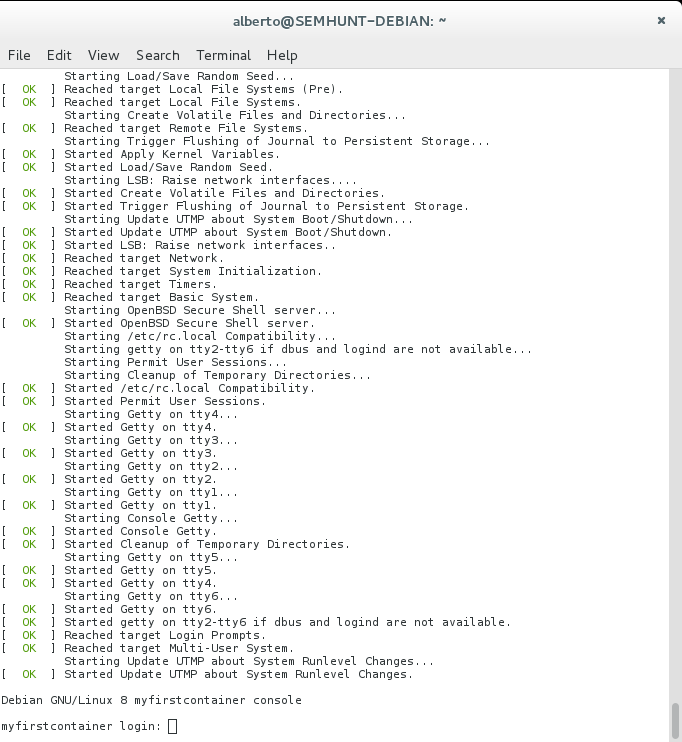
\includegraphics[width=0.9\textwidth]{14.png}
		\caption{Arrancando el Contenedor }
	\end{center}
\end{figure}

De igual form se puede arrancar un contenedor en segundo plano (no entra en él):

\begin{center}\shadowbox{lxc-start -n minigentoo -d.}\end{center}

Puedo ver su estado ahora:

\begin{center}\shadowbox{ sudo lxc-info -n minigentoo      (me informa de que está funcionando, pero estoy fuera).}\end{center}

Ahora bien, puedo ver los contenedores creados y su estado:
\begin{center}\shadowbox{ sudo lxc-ls -f.}\end{center}

\newpage

\begin{figure}[!ht]
	\begin{center}
		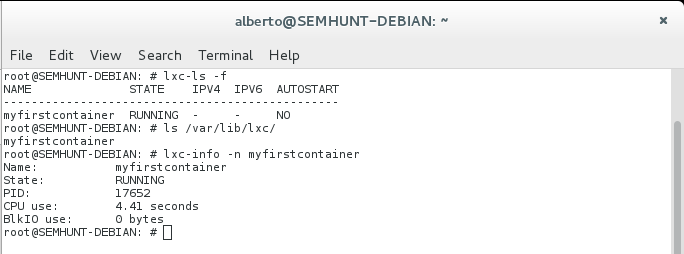
\includegraphics[width=0.9\textwidth]{17.png}
		\caption{Contenedores creados }
	\end{center}
\end{figure}
\begin{figure}[!ht]
	\begin{center}
		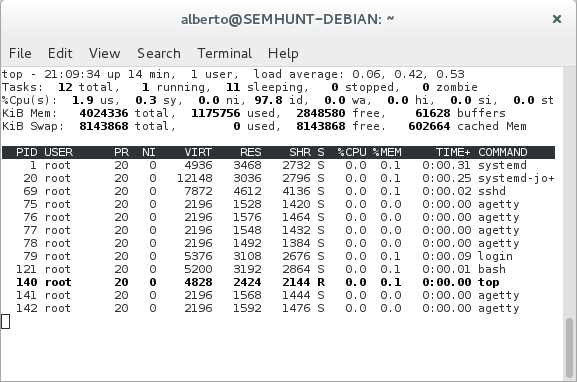
\includegraphics[width=0.9\textwidth]{18.png}
		\caption{Procesos del Contenedor }
	\end{center}
\end{figure}

\section{Configuración de Red}

Estaré usando libvirt para administrar el puente de red que vamos a crear para nuestros contenedores . Comienzo por habilitar la configuración de red por defecto que viene con libvirt:
\begin{center}\shadowbox{ sudo virsh -c lxc:/// net-define /etc/libvirt/qemu/networks/default.xml.}\end{center}
\begin{center}\shadowbox{ sudo virsh -c lxc:/// net-start default.}\end{center}
\begin{center}\shadowbox{ sudo virsh -c lxc:/// net-autostart default.}\end{center}

La red por defecto usando libvirt es 192.168.122.0/24 . Si desea cambiarlo , ejecute virsh -c lxc : /// net- edición por defecto y adaptar los ajustes.

\newpage

Ahora, estando el puente definido, necesito asignar ka interface de red a mi contenedor, hice esto agregando las siguientes lineas a /var/lib/lxc/myfirstcontainer/config

\begin{figure}[!ht]
	\begin{center}
		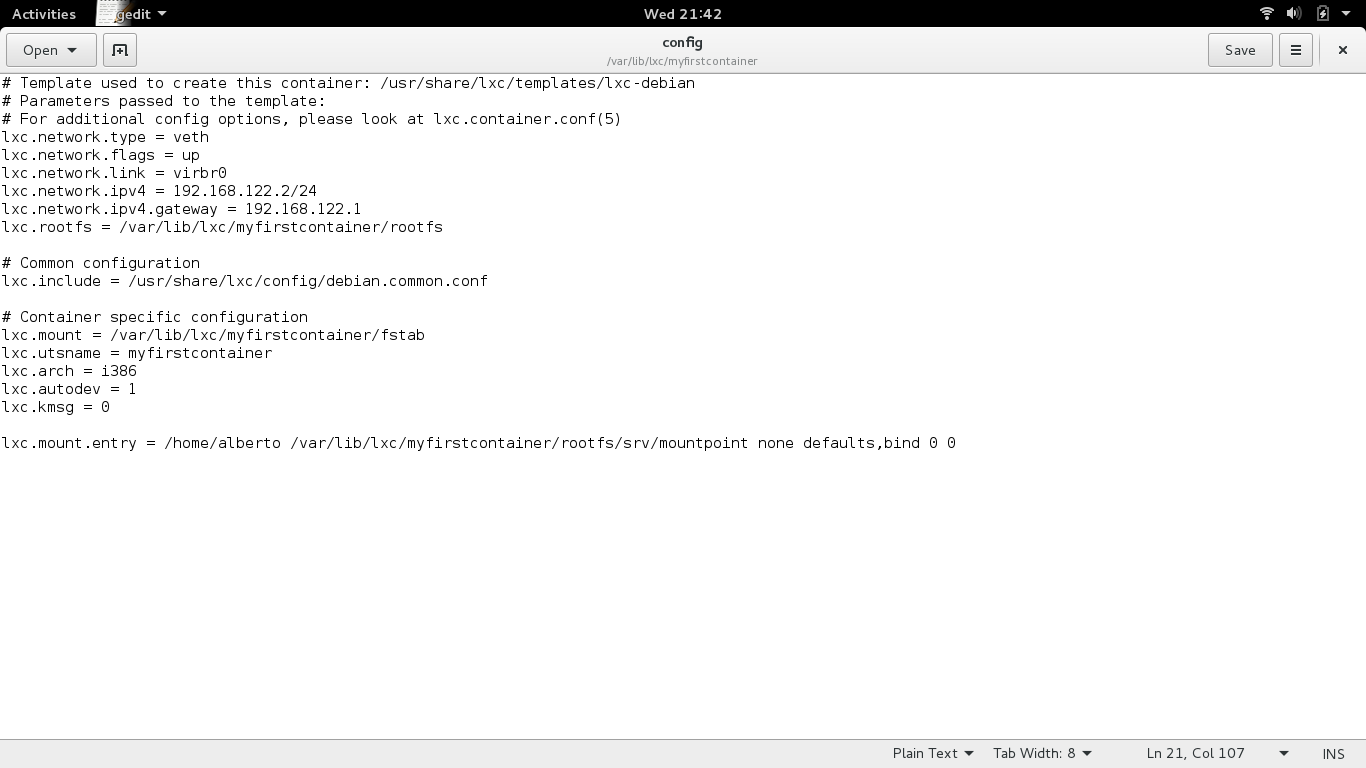
\includegraphics[width=0.9\textwidth]{20.png}
		\caption{Configuracion de Red }
	\end{center}
\end{figure}

\section{Iniciación Automática del Contenedor.}

Para iniciar automaticamente el contenedor desde que se inicia el boot, lo que teneos que hacer es colocar una ligaa los archivos de configuracion de nuestro contenedor a la siguiente ruta /etc/lxc/auto/

\begin{center}\shadowbox{ sudo ln -s /var/lib/lxc/myfirstcontainer/config /etc/lxc/auto/myfirstcontainer.}\end{center}

\section{Conclusión.}

Jamás había escuchado el término de Linux Containers, resolví muchos problemas creando máquinas virtuales lo que me tomaba mas tiempo y costo, el tener contenedores bien administrados me da ideas infinitas de poder hacer muchas cosas usando LXC, como por ejemplo tener una Base de Datos en un contenedor y un aplicativo web en otro contenedor. \\

Es extremadamamente conveniente poder tener varios sistemas heterogéneos funcionando en un servidor, pero no tener que preocuparse de configuraciones o versiones de lenguajes potencialmente conflictivas. Incluso el servir diferentes apps en la web a través de un proxy y simplifica las cosas. \\

Tomemos en cuenta que un contenedor tiene su propio sistema de ficheros y que es simplemente un directorio en nuestras máquinaa, así que puedemos hacer un rsync de eso a otra máquina, si quieremos copiar nuestro contenedor a otra máquina.\\

LXC está muy bien. El aislamiento es bueno.\\

\newpage

Ahora bien, resolviendo los puntos de esta tarea puedo comentar lo siguiente:\\

¿Pueden detectar como se ven diferentes procesos init desde el anfitrión?\\

R: No, lo que si pude detectar es que el contenedor maneja el mismo PID de systemd, pero por la caracteristica de LXC, este es un entorno con su propio espacio de procesos. Ahora, revisando los procesos de la maquina anfitrión, procesos como ssh, apache, etc, no comparten el mismo PID.\\

¿Pueden detectar cuantos y cuales procesos se ven desde el invitado?\\

R: No, de hecho podría atreverme a decir que es un ambiente aislado y esto hace que, el sistema operativo virtualizado, funcione a velocidad nativa, cosa que no ocurriría si hubiese que emular una máquina completa y tener varias instancias de kernels. En este sentido, podríamos considerarlos a los clásicos chroot, permitiendo más aislamiento y más flexibilidad.

¿Qué otras llamadas al sistema importantes creen que pasan para inicializar el contenedor?\\

R: Creo que las llamadas al sistema que realiza nuestro contenedor se realizan a los procesos de nuestro contenedor y a su vez directamente al kernel de la máquina anfitrión.

\end{document}










































